% Written with Elsevier's elsarticle LaTeX template (elsarticle.cls),
% the template for the Journal of Financial Economics and other Elsevier journals.
\documentclass[preprint,letterpaper,11pt,authoryear]{elsarticle}
\usepackage{lmodern}
\usepackage[margin=1in]{geometry}
\usepackage{amsmath}
\usepackage{graphicx}
\usepackage{booktabs}
\usepackage{array}
\usepackage[hidelinks]{hyperref}
\hypersetup{pdftitle={Do the Largest Firms' Earnings Move the S\&P 500?},pdfauthor={Nowshed Hossain Imran}}

% Notes printed under a table or figure
\newenvironment{tablenotes}{\par\vspace{3pt}\begin{minipage}{0.95\linewidth}\footnotesize\textit{Note:} }{\end{minipage}}
\newenvironment{figurenotes}{\par\vspace{3pt}\begin{minipage}{0.95\linewidth}\footnotesize\textit{Note:} }{\end{minipage}}

% Footer on the first page
\myfooter[L]{Course project, FIN 5633 Computational Finance, Oklahoma State University, revised October 2026}

\begin{document}

% let tables share a page with text instead of sitting alone on a float page
\renewcommand{\topfraction}{0.9}
\renewcommand{\textfraction}{0.1}
\renewcommand{\floatpagefraction}{0.8}

\begin{frontmatter}

\title{Do the Largest Firms' Earnings Move the S\&P 500? Evidence from Twenty Years of Earnings Announcements}

\author{Nowshed Hossain Imran}
\affiliation{organization={Spears School of Business, Oklahoma State University},
             city={Stillwater},
             state={OK},
             country={USA}}

\begin{abstract}
A few very large firms now make up a big share of the S\&P 500. I test whether the index moves more on days when a firm with 1\% or more of the index weight (a Big firm) reports earnings, using all 5,029 trading days from October 2006 to September 2026 and the 502 current constituents. Before reading the results I check that the data are suitable for regression and test the model's conditions. The errors are related from one day to the next and their spread is not constant, so I use Newey-West standard errors. Holding the previous day's VIX, the year and the month fixed, the index moves about 0.07 percentage points (about 9\%) more on Big-firm days than on days without reports ($p =$ 0.032), and more than on days when only smaller firms report ($p =$ 0.007). The effect grows with firm size and holds without 2008 and 2020. Misses by Big firms move the index more than beats, but this mostly comes from the two crisis years.
\end{abstract}

\begin{keyword}
Earnings announcements \sep S\&P 500 \sep Index concentration \sep Newey-West
\JEL G14 \sep C22
\end{keyword}

\end{frontmatter}

\section{Question and Main Findings}

Do earnings announcements of the largest S\&P 500 firms move the index more than announcements of everyone else? They do, modestly. On days when a firm with 1\% or more of the index reports, the index moves about 0.07 percentage points more than on days without reports, and the effect roughly doubles when the cutoff is raised to 2\%. Days when only smaller firms report look the same as days without any report.

The question matters because the S\&P 500 is weighted by market value, and its weight has become concentrated in a few very large firms. When one firm carries several percent of the index, news about that firm alone can move the index, and earnings announcements are the most regular source of such news. I test two hypotheses:

\begin{itemize}
  \item H1. The index moves more (in absolute terms) on days when a Big firm reports than on days with no reports or with only Small-firm reports.
  \item H2. Earnings misses by Big firms move the index more than Big beats of the same size.
\end{itemize}

The study began as a course project. In this revision I rebuilt it around the steps for time series regression I learned in econometrics (Wooldridge 2020): check the data, set up the model, test its conditions, choose the matching fix, and test whether the crisis years are different. The first version also tried to predict the direction of the index from earnings news. I dropped that part, because it is a forecasting exercise and does not fit these steps.

\section{Data and Method}

\subsection{Data}
I start from the 503 current S\&P 500 constituents listed on Wikipedia. One of them has no price data in the sample window, leaving 502 firms. Daily closing prices for each firm, the index (\^{}GSPC) and the VIX cover October 2006 to September 2026. Earnings dates, the time of each announcement and the EPS surprise against the analyst consensus come from Yahoo Finance through the yfinance library. I cap surprises at plus and minus 100\%, since firms with earnings close to zero can show huge percentage surprises. One Python script downloads the data, builds the sample and runs every test.

\subsection{Big and Small Firms}
A firm's market value on a day is its closing price times its current shares outstanding, and its index weight is that value divided by the total of all 502 firms. A firm counts as Big on an announcement if its weight was 1\% or more on the trading day before the market reacts. Using the day before keeps the announcement itself from deciding the group, and it lets a firm move between groups over the years.

\subsection{Reaction Day and Daily Variables}
Announcements at or after 4:00 p.m. Eastern time are assigned to the next trading day, since the market can react only when it reopens. Announcements before the open or during trading hours are assigned to the same day. Each trading day is then a Big day (at least one Big report), a Small-only day, or a day without reports. The first version used earnings days only. However, the revision keeps all 5,029 trading days, so the data form one unbroken daily series: 944 Big days, 2,865 Small-only days and 1,220 days without reports.

\subsection{Checking the Data}
A regression on daily data can be trusted only if the series do not wander off without returning to a normal level (Wooldridge 2020). Figure 1, panel (a), shows the absolute index return. It comes in clusters, with long calm stretches and short violent ones in 2008 and 2020, but it always comes back to its usual level. Table 1 confirms this. Today's absolute return is related to yesterday's with a coefficient of 0.31, far below one, and the Dickey-Fuller test rejects a unit root for all three series. The VIX is very persistent (0.97), still it returns to its average as well. Therefore, the data are suitable for regression.

\begin{table}[!htbp]
\centering\small\setlength{\tabcolsep}{4pt}
\caption{Do the Series Return to a Normal Level?}
\begin{tabular}{lccc}
\toprule
Series & Link to previous day & Dickey-Fuller & $p$-value \\
\midrule
Daily index return (\%) & $-$0.12 & $-$16.23 & $<$ 0.001 \\
Absolute index return (\%) & 0.31 & $-$6.75 & $<$ 0.001 \\
VIX (previous day) & 0.97 & $-$5.76 & $<$ 0.001 \\
\bottomrule
\end{tabular}
\begin{tablenotes}
Link to previous day: coefficient from a regression of each series on its own previous value. A value well below one means the series returns to its usual level. A small Dickey-Fuller $p$-value means the same. All 5,029 trading days.
\end{tablenotes}
\end{table}

\subsection{Model}
For H1, I regress the absolute index return (\%) on a Big-day dummy and a Small-day dummy, so days without reports are the comparison group:
\begin{equation}
|r_t| = \beta_0 + \beta_1\,\text{Big}_t + \beta_2\,\text{Small}_t + \beta_3\,\text{VIX}_{t-1} + \text{year dummies} + \text{month dummies} + u_t
\end{equation}
H1 predicts $\beta_1 > 0$ and $\beta_1 > \beta_2$. Each control has a reason. In a nervous market the index moves more, and large firms may also be more likely to disappoint, so I control for the VIX. Today's VIX moves together with today's return, so I use the previous day's VIX, which is known before the day begins. Year dummies compare days within the same year, so calm and turbulent years do not drive the result. Month dummies deal with seasons (Wooldridge 2020): earnings arrive in seasons, and January, April, July and October could be more volatile for reasons that has nothing to do with any single firm.

\subsection{Testing the Model's Conditions}
Before trusting the standard errors, I test the conditions of the time series model (Table 2). The errors are related from one day to the next (serial correlation): the AR(1) coefficient is $-$0.08 and the Breusch-Godfrey test rejects ($p <$ 0.001). Their spread is also not constant (heteroskedasticity, Breusch-Pagan $p <$ 0.001). The last check is strict exogeneity, which asks whether future values of the regressors are related to today's error. I add the next day's value of each regressor. Tomorrow's VIX is clearly significant ($t$ = 7.0), which makes sense, because a big move today raises tomorrow's VIX. Tomorrow's Big day is not significant, as expected, since earnings dates are set well in advance.

\begin{table}[!htbp]
\centering\small\setlength{\tabcolsep}{4pt}
\caption{Tests of the H1 Model's Conditions}
\begin{tabular}{llcc}
\toprule
Condition & Test & Statistic & $p$-value \\
\midrule
Right functional form & RESET & $F = 10.67$ & $<$ 0.001 \\
No serial correlation & AR(1) on residuals & $\hat\rho = -0.076$ & $<$ 0.001 \\
 & Breusch-Godfrey, 9 lags & 138.9 & $<$ 0.001 \\
Constant error spread & Breusch-Pagan & 895.1 & $<$ 0.001 \\
Strict exogeneity & Next day's VIX ($t$) & 7.00 & $<$ 0.001 \\
 & Next day's Big day ($t$) & 0.39 & 0.695 \\
\bottomrule
\end{tabular}
\begin{tablenotes}
Tests on the OLS residuals of the H1 model with the previous day's VIX, year dummies and month dummies. A small $p$-value means the condition fails. $n$ = 5,029 trading days.
\end{tablenotes}
\end{table}

With these problems, the OLS coefficients are still fine in a large sample, but the usual standard errors are wrong. There are two common fixes (Wooldridge 2020). Prais-Winsten FGLS transforms the data to remove the serial correlation and gives more precise estimates, but it needs strict exogeneity. Newey-West standard errors keep the OLS coefficients and only correct the standard errors, for both serial correlation and unequal spread, and they do not need strict exogeneity. Since strict exogeneity fails here, Newey-West is the right choice. I use it for all main results, with 9 lags from the usual rule of thumb, and report Prais-Winsten only for comparison.

The RESET test says the linear model does not capture everything ($p <$ 0.001). I tried the usual remedies: adding the squared VIX, using the log of the VIX, and adding yesterday's absolute return. RESET rejects in every version, which is not surprising for daily returns with many extreme days over 5,000 days. However, the Big-day coefficient stays between 0.070 and 0.077 and remains significant in all of them, so this does not change the answer to H1.

\subsection{H2 and the Crisis Years}
For H2, I multiply each surprise by the firm's weight, so a 5\% beat by a firm with 6\% weight counts more than the same beat by a small firm. I split it into a beat part (zero or above) and a miss part (zero or below) and add each part up by day. I then regress the daily index return on Big beats, Big misses, Small beats and Small misses, with the same controls and Newey-West standard errors. Misses are negative numbers, so a positive coefficient on misses means larger misses go with lower index returns. A one-sided test checks whether the Big-miss coefficient is larger than the Big-beat coefficient. For both hypotheses, a Chow-style test (Wooldridge 2020) checks whether the key effects are different in 2008 and 2020.

\section{Results}

\subsection{H1: Size of Index Moves}
Table 3 shows the raw pattern. The index moves 0.844\% on average on Big days, against 0.777\% on Small-only days and 0.783\% on days with no reports, so Small-only days look just like days without earnings news.

\begin{table}[!htbp]
\centering\small\setlength{\tabcolsep}{4pt}
\caption{Average Absolute Daily Index Return by Day Type}
\begin{tabular}{lcc}
\toprule
Day type & Days & Mean $|$return$|$ (\%) \\
\midrule
No earnings reports & 1,220 & 0.783 \\
Small firms only & 2,865 & 0.777 \\
At least one Big firm & 944 & 0.844 \\
\bottomrule
\end{tabular}
\begin{tablenotes}
Big days use the 1\% cutoff.
\end{tablenotes}
\end{table}

Table 4 gives the H1 regression. With the controls, the Big-day coefficient is 0.072, about 9\% of the typical absolute move on a day without reports, while the Small-day coefficient is close to zero ($-$0.006). Without controls it is 0.061, so taking market conditions into account makes the effect slightly larger, not smaller. The month dummies are not jointly significant ($p =$ 0.19), so earnings seasons are not more volatile overall. With Newey-West standard errors the Big-day effect has $p =$ 0.032, and it is significantly larger than the Small-day effect ($p =$ 0.007). Prais-Winsten gives almost the same estimate (0.073), which is reassuring even though it is not the preferred method here.

\begin{table}[!htbp]
\centering\small\setlength{\tabcolsep}{4pt}
\caption{H1: Big-Day Effect on the Absolute Index Return}
\begin{tabular}{lcccc}
\toprule
Method & Big day & Std.\ error & $p$-value & Big $-$ Small, $p$ \\
\midrule
OLS, usual standard errors & 0.072 & 0.036 & 0.043 & 0.011 \\
OLS, robust (HC1) & 0.072 & 0.036 & 0.044 & 0.010 \\
OLS, Newey-West (main) & 0.072 & 0.034 & 0.032 & 0.007 \\
Prais-Winsten FGLS & 0.073 & 0.035 & 0.035 & 0.009 \\
\bottomrule
\end{tabular}
\begin{tablenotes}
Dependent variable: absolute daily index return (\%). All models include the previous day's VIX, year dummies and month dummies ($n$ = 5,029). The Big-day coefficient is the extra absolute return compared with days without reports. Two-sided $p$-values.
\end{tablenotes}
\end{table}

\subsection{Firm Size and the Crisis Years}
Table 5 shows how the effect depends on firm size and on the crisis years. It is 0.036 and not significant with a 0.5\% cutoff, 0.072 at 1\%, and 0.152 at 2\%. The larger the reporting firms, the larger the index move, which is what H1 predicts. The Chow-style test finds no change in the day-type effects in 2008 and 2020 ($p =$ 0.31), and without those two years the Big-day effect is 0.095 ($p =$ 0.002). So the result is not just crisis volatility.

\begin{table}[!htbp]
\centering\small\setlength{\tabcolsep}{4pt}
\caption{H1 by Cutoff and Without the Crisis Years}
\begin{tabular}{lccc}
\toprule
Specification & Big days & Big-day effect & $p$-value \\
\midrule
Cutoff 0.5\% & 1,666 & 0.036 & 0.225 \\
Cutoff 1\% (main) & 944 & 0.072 & 0.032 \\
Cutoff 2\% & 272 & 0.152 & 0.009 \\
Excluding 2008 and 2020 &  & 0.095 & 0.002 \\
Chow-style test, 2008 and 2020 &  &  & 0.308 \\
\bottomrule
\end{tabular}
\begin{tablenotes}
OLS with Newey-West standard errors and all controls. The last row tests whether the Big-day and Small-day effects both stay the same in 2008 and 2020.
\end{tablenotes}
\end{table}

\subsection{H2: Misses versus Beats}
Over all years, the Big-miss coefficient is 0.41 and the Big-beat coefficient is small and negative ($-$0.10), so the difference is 0.51 (one-sided $p <$ 0.001). In practical terms, a 5\% miss by a firm with 6\% index weight (0.30 units) goes with an index return about 0.12 percentage points lower. However, without 2008 and 2020 the difference falls to 0.26 and is no longer significant ($p =$ 0.10), and the Chow-style test cannot tell whether the effects differ in those years ($p =$ 0.18). The data therefore cannot separate the asymmetry from the two crises. From a value-investing standpoint, a result that depends on two years has little margin of safety.

\begin{table}[!htbp]
\centering\small\setlength{\tabcolsep}{4pt}
\caption{H2: Big-Miss Effect Minus Big-Beat Effect}
\begin{tabular}{lcccc}
\toprule
Sample & Big beat & Big miss & Difference & $p$-value \\
\midrule
All years & $-$0.099 & 0.412 & 0.511 & $<$ 0.001 \\
Excluding 2008 and 2020 & $-$0.062 & 0.201 & 0.263 & 0.105 \\
Chow-style test, 2008 and 2020 &  &  &  & 0.175 \\
\bottomrule
\end{tabular}
\begin{tablenotes}
Dependent variable: daily index return (\%). Regressors are weight-scaled beats and misses for Big and Small firms, with the same controls and Newey-West standard errors. One-sided $p$-values for the difference; joint $F$-test for the Chow row.
\end{tablenotes}
\end{table}

\begin{figure}[!htbp]
\centering
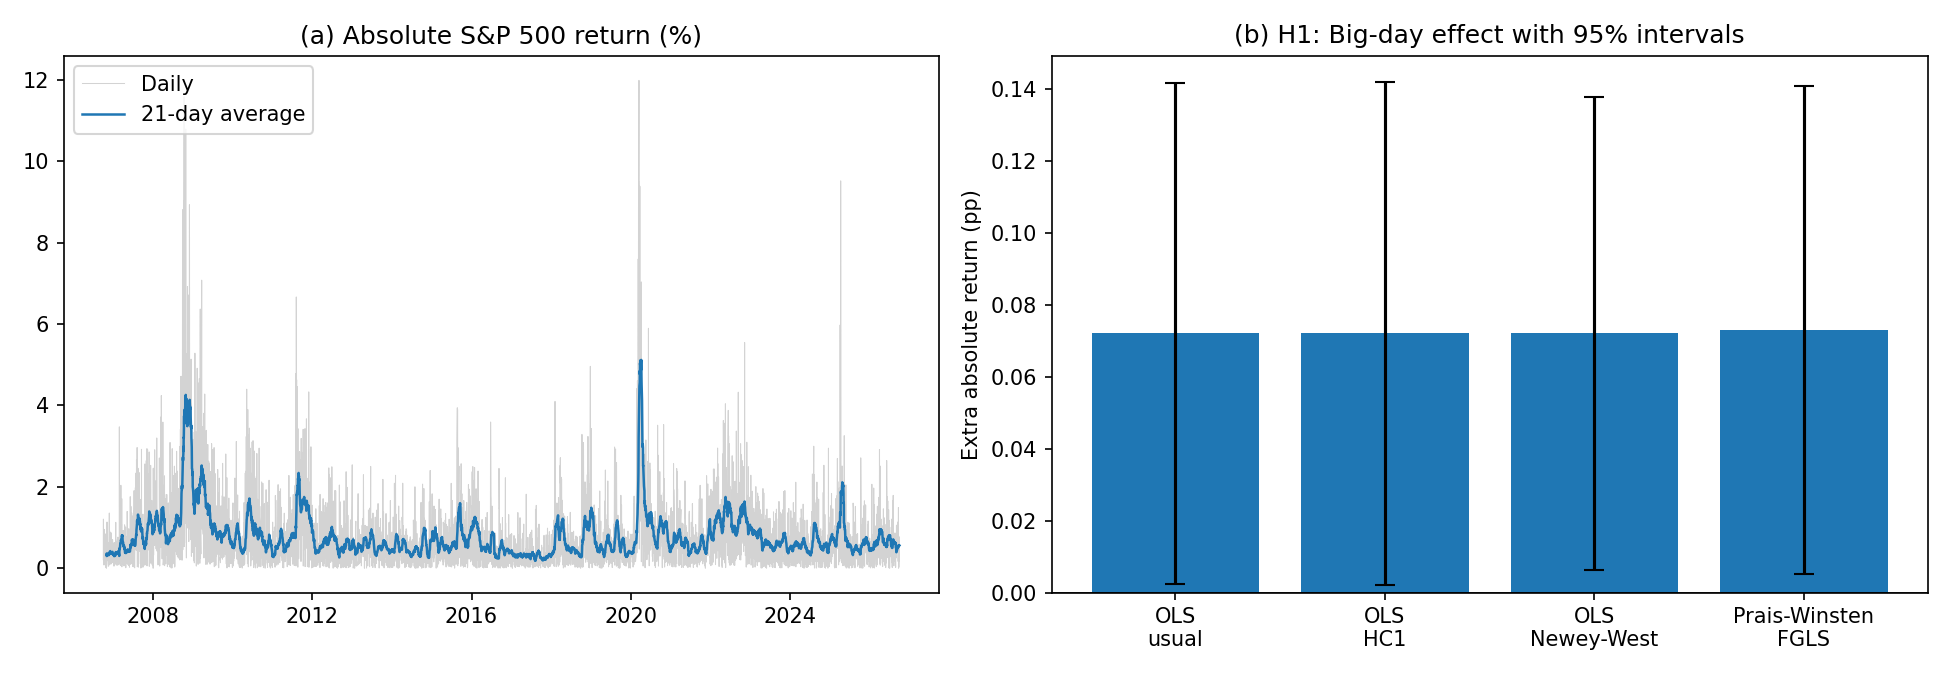
\includegraphics[width=\linewidth]{results.png}
\caption{Absolute Index Return and the H1 Estimates}
\begin{figurenotes}
Panel (a): absolute daily S\&P 500 return with its 21-day average. Panel (b): H1 Big-day effect with 95\% confidence intervals under each method.
\end{figurenotes}
\end{figure}

\section{Limitations}
\begin{itemize}
  \item Only current constituents are included, so firms that left the index during the sample are missing (survivorship bias).
  \item Index weights use today's shares outstanding for every year and are not float-adjusted.
  \item Daily close-to-close returns include the overnight move, and they cannot separate the reaction to one announcement when several firms report on the same day.
  \item The model fails the RESET test. The Big-day effect is stable in every alternative I tried, but the model is still a simplification.
  \item Earnings histories from Yahoo Finance are less complete in the earlier years.
\end{itemize}

\section{Conclusion}
Following the econometric steps changed the study more than any single test. Checking the data first showed that a regression was appropriate, testing the conditions showed that the usual standard errors could not be trusted, and the strict exogeneity test decided between the two fixes. With those choices made in order, the main result became cleaner than in the first version: earnings days of the largest S\&P 500 firms come with larger index moves, the effect grows with firm size, and it does not depend on 2008 and 2020. The miss-versus-beat asymmetry, on the other hand, cannot be separated from the crises. Natural next steps are to use the historical index membership to remove survivorship bias and to look at intraday prices around each announcement. Without passing the assumption tests, a number, however good it looks on paper, cannot indicate a causal relationship.

\begin{thebibliography}{00}
\bibitem[Wooldridge(2020)]{wooldridge} Wooldridge, Jeffrey M. 2020. \textit{Introductory Econometrics: A Modern Approach}. 7th ed. Boston: Cengage.
\end{thebibliography}

\vspace{6pt}
\noindent Code: \href{https://github.com/nowshed-imran/FIN-5633-Project}{github.com/nowshed-imran/FIN-5633-Project}

\end{document}
